\documentclass[12pt,]{article}
\usepackage[left=1in,top=1in,right=1in,bottom=1in]{geometry}
\newcommand*{\authorfont}{\fontfamily{phv}\selectfont}
\usepackage[]{mathpazo}


  \usepackage[T1]{fontenc}
  \usepackage[utf8]{inputenc}




\usepackage{abstract}
\renewcommand{\abstractname}{}    % clear the title
\renewcommand{\absnamepos}{empty} % originally center

\renewenvironment{abstract}
 {{%
    \setlength{\leftmargin}{0mm}
    \setlength{\rightmargin}{\leftmargin}%
  }%
  \relax}
 {\endlist}

\makeatletter
\def\@maketitle{%
  \newpage
%  \null
%  \vskip 2em%
%  \begin{center}%
  \let \footnote \thanks
    {\fontsize{18}{20}\selectfont\raggedright  \setlength{\parindent}{0pt} \@title \par}%
}
%\fi
\makeatother




\setcounter{secnumdepth}{0}

\usepackage{longtable,booktabs}

\usepackage{graphicx,grffile}
\makeatletter
\def\maxwidth{\ifdim\Gin@nat@width>\linewidth\linewidth\else\Gin@nat@width\fi}
\def\maxheight{\ifdim\Gin@nat@height>\textheight\textheight\else\Gin@nat@height\fi}
\makeatother
% Scale images if necessary, so that they will not overflow the page
% margins by default, and it is still possible to overwrite the defaults
% using explicit options in \includegraphics[width, height, ...]{}
\setkeys{Gin}{width=\maxwidth,height=\maxheight,keepaspectratio}


\title{Political Donor Motivations and Social Media: A Time-Series Analysis  }



\author{\Large \vspace{0.05in} \newline\normalsize\emph{}  }


\date{}

\usepackage{titlesec}

\titleformat*{\section}{\normalsize\bfseries}
\titleformat*{\subsection}{\normalsize\itshape}
\titleformat*{\subsubsection}{\normalsize\itshape}
\titleformat*{\paragraph}{\normalsize\itshape}
\titleformat*{\subparagraph}{\normalsize\itshape}





\newtheorem{hypothesis}{Hypothesis}
\usepackage{setspace}


% set default figure placement to htbp
\makeatletter
\def\fps@figure{htbp}
\makeatother

\usepackage{graphicx}

% move the hyperref stuff down here, after header-includes, to allow for - \usepackage{hyperref}

\makeatletter
\@ifpackageloaded{hyperref}{}{%
\ifxetex
  \PassOptionsToPackage{hyphens}{url}\usepackage[setpagesize=false, % page size defined by xetex
              unicode=false, % unicode breaks when used with xetex
              xetex]{hyperref}
\else
  \PassOptionsToPackage{hyphens}{url}\usepackage[draft,unicode=true]{hyperref}
\fi
}

\@ifpackageloaded{color}{
    \PassOptionsToPackage{usenames,dvipsnames}{color}
}{%
    \usepackage[usenames,dvipsnames]{color}
}
\makeatother
\hypersetup{breaklinks=true,
            bookmarks=true,
            pdfauthor={ ()},
             pdfkeywords = {},  
            pdftitle={Political Donor Motivations and Social Media: A Time-Series Analysis},
            colorlinks=true,
            citecolor=blue,
            urlcolor=blue,
            linkcolor=magenta,
            pdfborder={0 0 0}}
\urlstyle{same}  % don't use monospace font for urls

% Add an option for endnotes. -----


% add tightlist ----------
\providecommand{\tightlist}{%
\setlength{\itemsep}{0pt}\setlength{\parskip}{0pt}}

% add some other packages ----------

% \usepackage{multicol}
% This should regulate where figures float
% See: https://tex.stackexchange.com/questions/2275/keeping-tables-figures-close-to-where-they-are-mentioned
\usepackage[section]{placeins}


\begin{document}
	
% \pagenumbering{arabic}% resets `page` counter to 1 
%
% \maketitle

{% \usefont{T1}{pnc}{m}{n}
\setlength{\parindent}{0pt}
\thispagestyle{plain}
{\fontsize{18}{20}\selectfont\raggedright 
\maketitle  % title \par  

}

{
   \vskip 13.5pt\relax \normalsize\fontsize{11}{12} 
\textbf{\authorfont } \hskip 15pt \emph{\small }   

}

}






\vskip -8.5pt


 % removetitleabstract

\noindent \doublespacing 

The two predominant theories of political donor motivations are the
access-oriented model (Fouirnaies and Hall 2015) and the consumption
model (Ansolabehere, Figueiredo, and Snyder 2003). In the
access-oriented model, individual political donors and political action
committees (PACs) are assumed to contribute to campaigns in an effort to
acquire access and influence politicians into supporting specific policy
issues (Fouirnaies and Hall 2015). The consumption model of donors views
political contributions as being an extension of voting along a
participatory spectrum, and that donors support candidates who they
already know support policy issues that the donors care about or are
ideologically motivated (Barber 2016; Johnson 2010). Previous studies
have posited these two models of political donor motivations against
each other (Heerwig 2016).

This paper combines political donation records and Twitter and Facebook
posts from politicians. These two datasets are analyzed together to
examine if politicians' public support of various policy issues on
social media precede, lag, or have no relationship with donations from
various communities of political donors. The access-oriented model of
political donors predicts that donations from specific groups of donors
will precede public support of certain policies. In contrast, the
consumption model of political donors predicts that donations from
various groups of donors would lag in response to public support of
certain policy issues by candidates. This paper sets these two models of
political donors against each other to see if evidence of either model
is found in observational data.

\hypertarget{data}{%
\section{Data}\label{data}}

Data for this research comes from two primary sources: politicians'
social media posts and political donation data. For social media posts,
this paper used the Facebook and Twitter APIs to collect social media
posts from all candidates for the Wisconsin State Senate and Wisconsin
State Assembly during the 2016 election cycle (\emph{n} = 82,851). A
subset of these posts were hand-coded into 27 topical categories. This
subset was used to train a BERT deep learning transfer model that was
used to predict the topic of the remainder of the posts (training
dataset = 8,242, 10\% of total posts; testing dataset = 4,122, 5\% of
total posts). Political donation data for all candidates to the
Wisconsin State Legislature during the 2016 election cycle were
collected from the Wisconsin Campaign Information System (CFIS). These
donations were used to create a network of political donations with
candidates and donors serving as nodes and donations between them as
edges. This network was clustered into distinct communities so that
donors in each community are most similar to one another based on which
campaigns they contributed to. I theorize that these clusters of donors
represent \emph{latent coalitions} of donors who, whether they operate
in an organized fashion or not, are working toward the goal of electing
the same candidates. Studying political fundraisers as members of
political coalitions has been studied in the past (Adams 2007; Heerwig
2016), and this paper's statistically-driven definition of latent
coalitions seeks to add to the coalition literature.

\hypertarget{methodology}{%
\section{Methodology}\label{methodology}}

These two datasets were analyzed against each other using the Granger
causality time-series methodology This methodology has been used by
other researchers to study social media (Freelon, McIlwain, and Clark
2018; Lukito 2020). Similar to political donations, this methodology has
been used to study non-social media events such as offline protests
(Bastos, Mercea, and Charpentier 2015) and stock prices (Park, Leung,
and Ma 2017). This methodology detects whether movements in one time
series precedes, lags, has a confounding variable, or is not related to
another time series. Specifically, this paper compares time series of
donations from clusters of political donors and times series of the
number of social media posts by each topic that were made by campaigns
that each donor cluster contributed to. For example, a time series of
donations from a donor cluster was compared to the aggregate count of
posts about a given topic made by candidates that the donor cluster
contributed to.

\hypertarget{results}{%
\section{Results}\label{results}}

Initial results provide some evidence consistent with both the
access-oriented and consumption models, but more coalitions of donors
exhibit behavior that is consistent with the consumption model of donor
motivations. In about 31\% (4/13) of coalitions, donations from the
coalition lagged social media posts about at least one specific topic by
the candidates that they donated to--behavior that is predicted by the
consumption model of donor motivations. About 15\% (2/13) of coalitions
showed behavior inline with the access-oriented model of donors where
their donations preceded social media posts about at least one specific
topic made by candidates that they contributed to. Specific results can
be found in Figure 1.

\begin{figure}
\centering
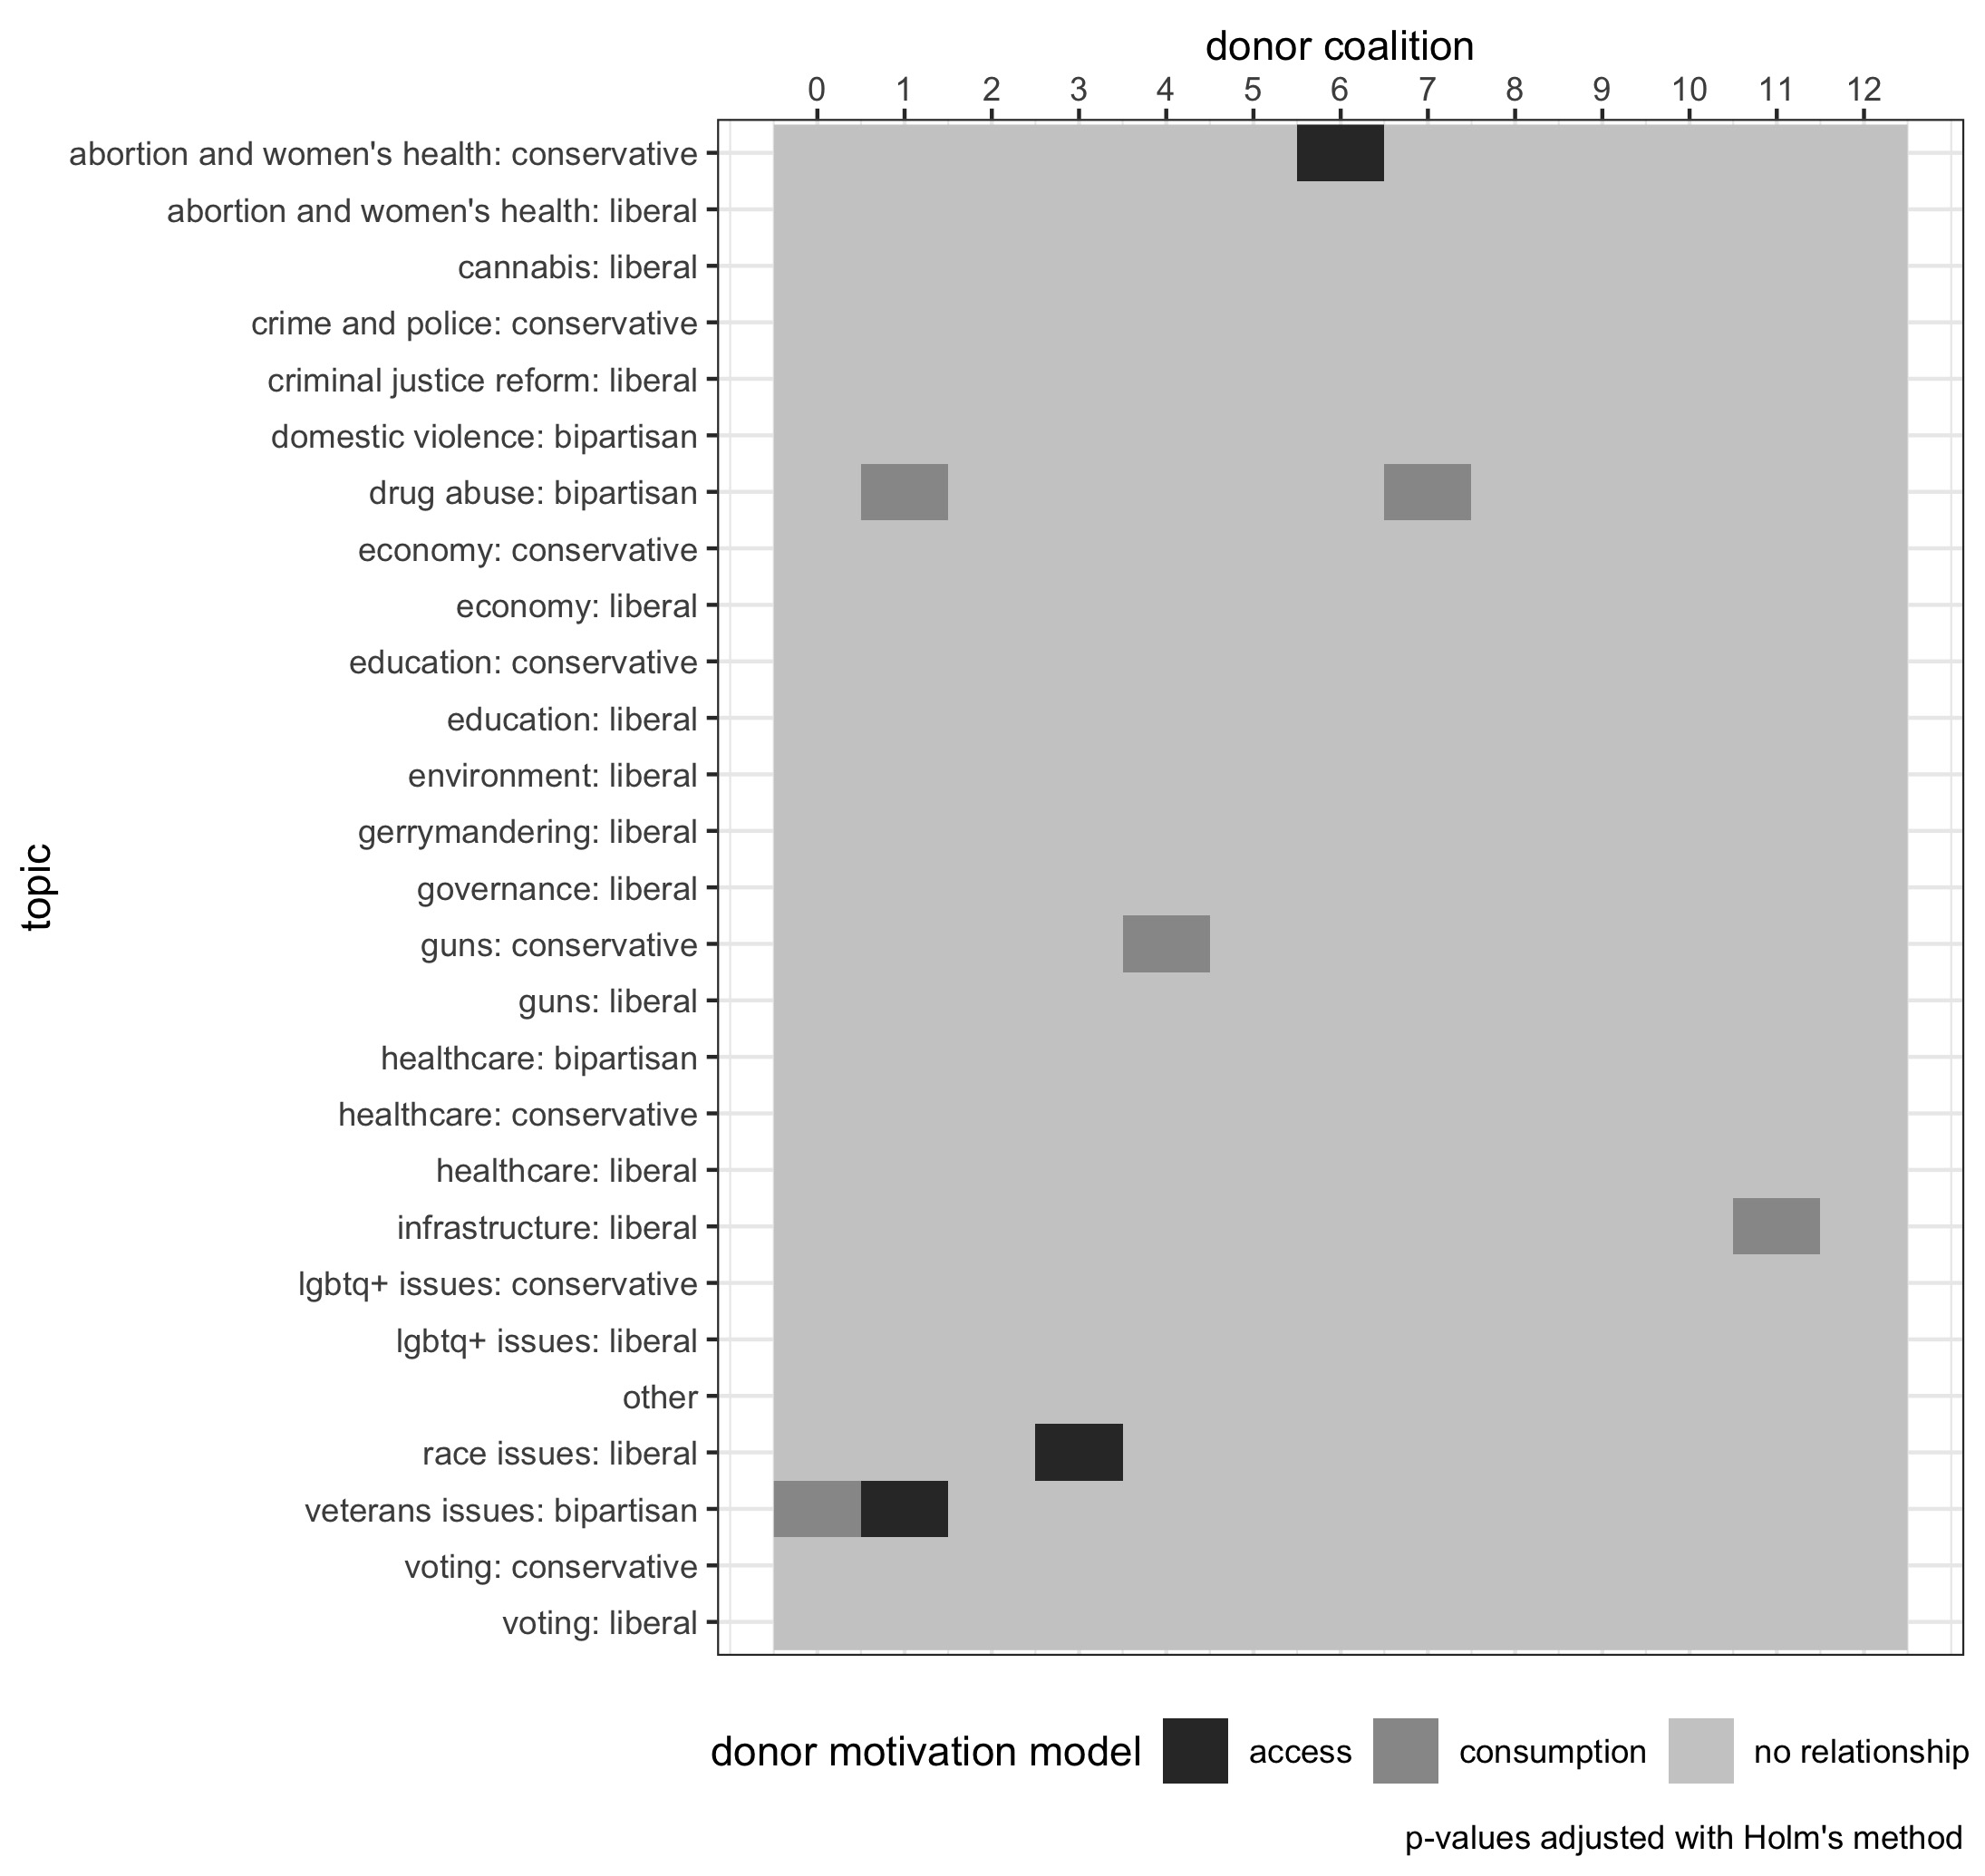
\includegraphics{../tables_and_figures/aejmc_abstract_1.jpg}
\caption{Donor Motivation Models}
\end{figure}

The next step is to analyze potential confounding factors that could
describe the motivations of political donors, such as geographic
proximity or competitiveness of the races the cluster contributed to in
aggregate. These factors are especially important for the coalitions
that the model identified as having a confounding variable or not having
a relationship.

\hypertarget{word-count}{%
\section{Word Count}\label{word-count}}

\begin{longtable}[]{@{}lll@{}}
\toprule
Method & koRpus & stringi\tabularnewline
\midrule
\endhead
Word count & 789 & 778\tabularnewline
Character count & 5240 & 5239\tabularnewline
Sentence count & 34 & Not available\tabularnewline
Reading time & 3.9 minutes & 3.9 minutes\tabularnewline
\bottomrule
\end{longtable}

\hypertarget{references}{%
\section*{References}\label{references}}
\addcontentsline{toc}{section}{References}

\hypertarget{refs}{}
\leavevmode\hypertarget{ref-adams2016}{}%
Adams, Brian E. 2007. ``Fundraising Coalitions in Open Seat Mayoral
Elections.'' \emph{Journal of Urban Affairs} 29 (5): 481--99.
\url{https://doi.org/10.1111/j.1467-9906.2007.00361.x}.

\leavevmode\hypertarget{ref-ansolabehere2003}{}%
Ansolabehere, Stephen, John M. de Figueiredo, and James M. Snyder. 2003.
``Why Is There so Little Money in U.s. Politics.'' \emph{Journal of
Economic Perspectives} 17 (1): 105--30.

\leavevmode\hypertarget{ref-barber2016}{}%
Barber, Michael. 2016. ``Donation Motivations: Testing Theories of
Access and Ideology.'' \emph{Political Research Quarterly} 69 (1):
148--59.

\leavevmode\hypertarget{ref-bastos2015}{}%
Bastos, Marco T., Dan Mercea, and Arthur Charpentier. 2015. ``Tents,
Tweets, and Events: The Interplay Between Ongoing Protests and Social
Media.'' \emph{Journal of Communication} 65 (2): 320--50.
\url{https://doi.org/10.1111/jcom.12145}.

\leavevmode\hypertarget{ref-fouirnaies2015}{}%
Fouirnaies, Alexander, and Andrew Hall. 2015. ``The Exposure Theory of
Access: Why Some Firms Seek More Access to Incumbents Than Others.''
\emph{SSRN Electronic Journal}, January.
\url{https://doi.org/10.2139/ssrn.2652361}.

\leavevmode\hypertarget{ref-freelon2018}{}%
Freelon, D, C McIlwain, and M Clark. 2018. ``Quantifying the Power and
Consequences of Social Media Protest.'' \emph{New Media \& Society} 20
(3): 990--1011. \url{https://doi.org/10.1177/1461444816676646}.

\leavevmode\hypertarget{ref-heerwig2016}{}%
Heerwig, Jennifer A. 2016. ``Donations and Dependence: Individual
Contributor Strategies in House Elections.'' \emph{Social Science
Research} 60: 181--98.
\url{https://doi.org/https://doi.org/10.1016/j.ssresearch.2016.06.001}.

\leavevmode\hypertarget{ref-johnson2010}{}%
Johnson, Bertram. 2010. ``Individual Contributions: A Fundraising
Advantage for the Ideologically Extreme?'' \emph{American Politics
Research}, June, 890--908.
\url{https://doi.org/10.1177/1532673X09357500}.

\leavevmode\hypertarget{ref-lukito2020}{}%
Lukito, Josephine. 2020. ``Coordinating a Multi-Platform Disinformation
Campaign: Internet Research Agency Activity on Three U.s. Social Media
Platforms, 2015 to 2017.'' \emph{Political Communication} 37 (2):
238--55. \url{https://doi.org/10.1080/10584609.2019.1661889}.

\leavevmode\hypertarget{ref-park2017}{}%
Park, J., H. Leung, and K. Ma. 2017. ``Information Fusion of Stock
Prices and Sentiment in Social Media Using Granger Causality.'' In
\emph{2017 Ieee International Conference on Multisensor Fusion and
Integration for Intelligent Systems (Mfi)}, 614--19.
\url{https://doi.org/10.1109/MFI.2017.8170390}.





\newpage
\singlespacing 
\end{document}
